%\chapter{\leavevmode Timeline}
% \chapter*{Timeline}
% \addcontentsline{toc}{chapter}{Timeline}
\chapter{\leavevmode Timeline}
\label{chap:timeline}

\begin{figure}[!htb]%
  \centering
  {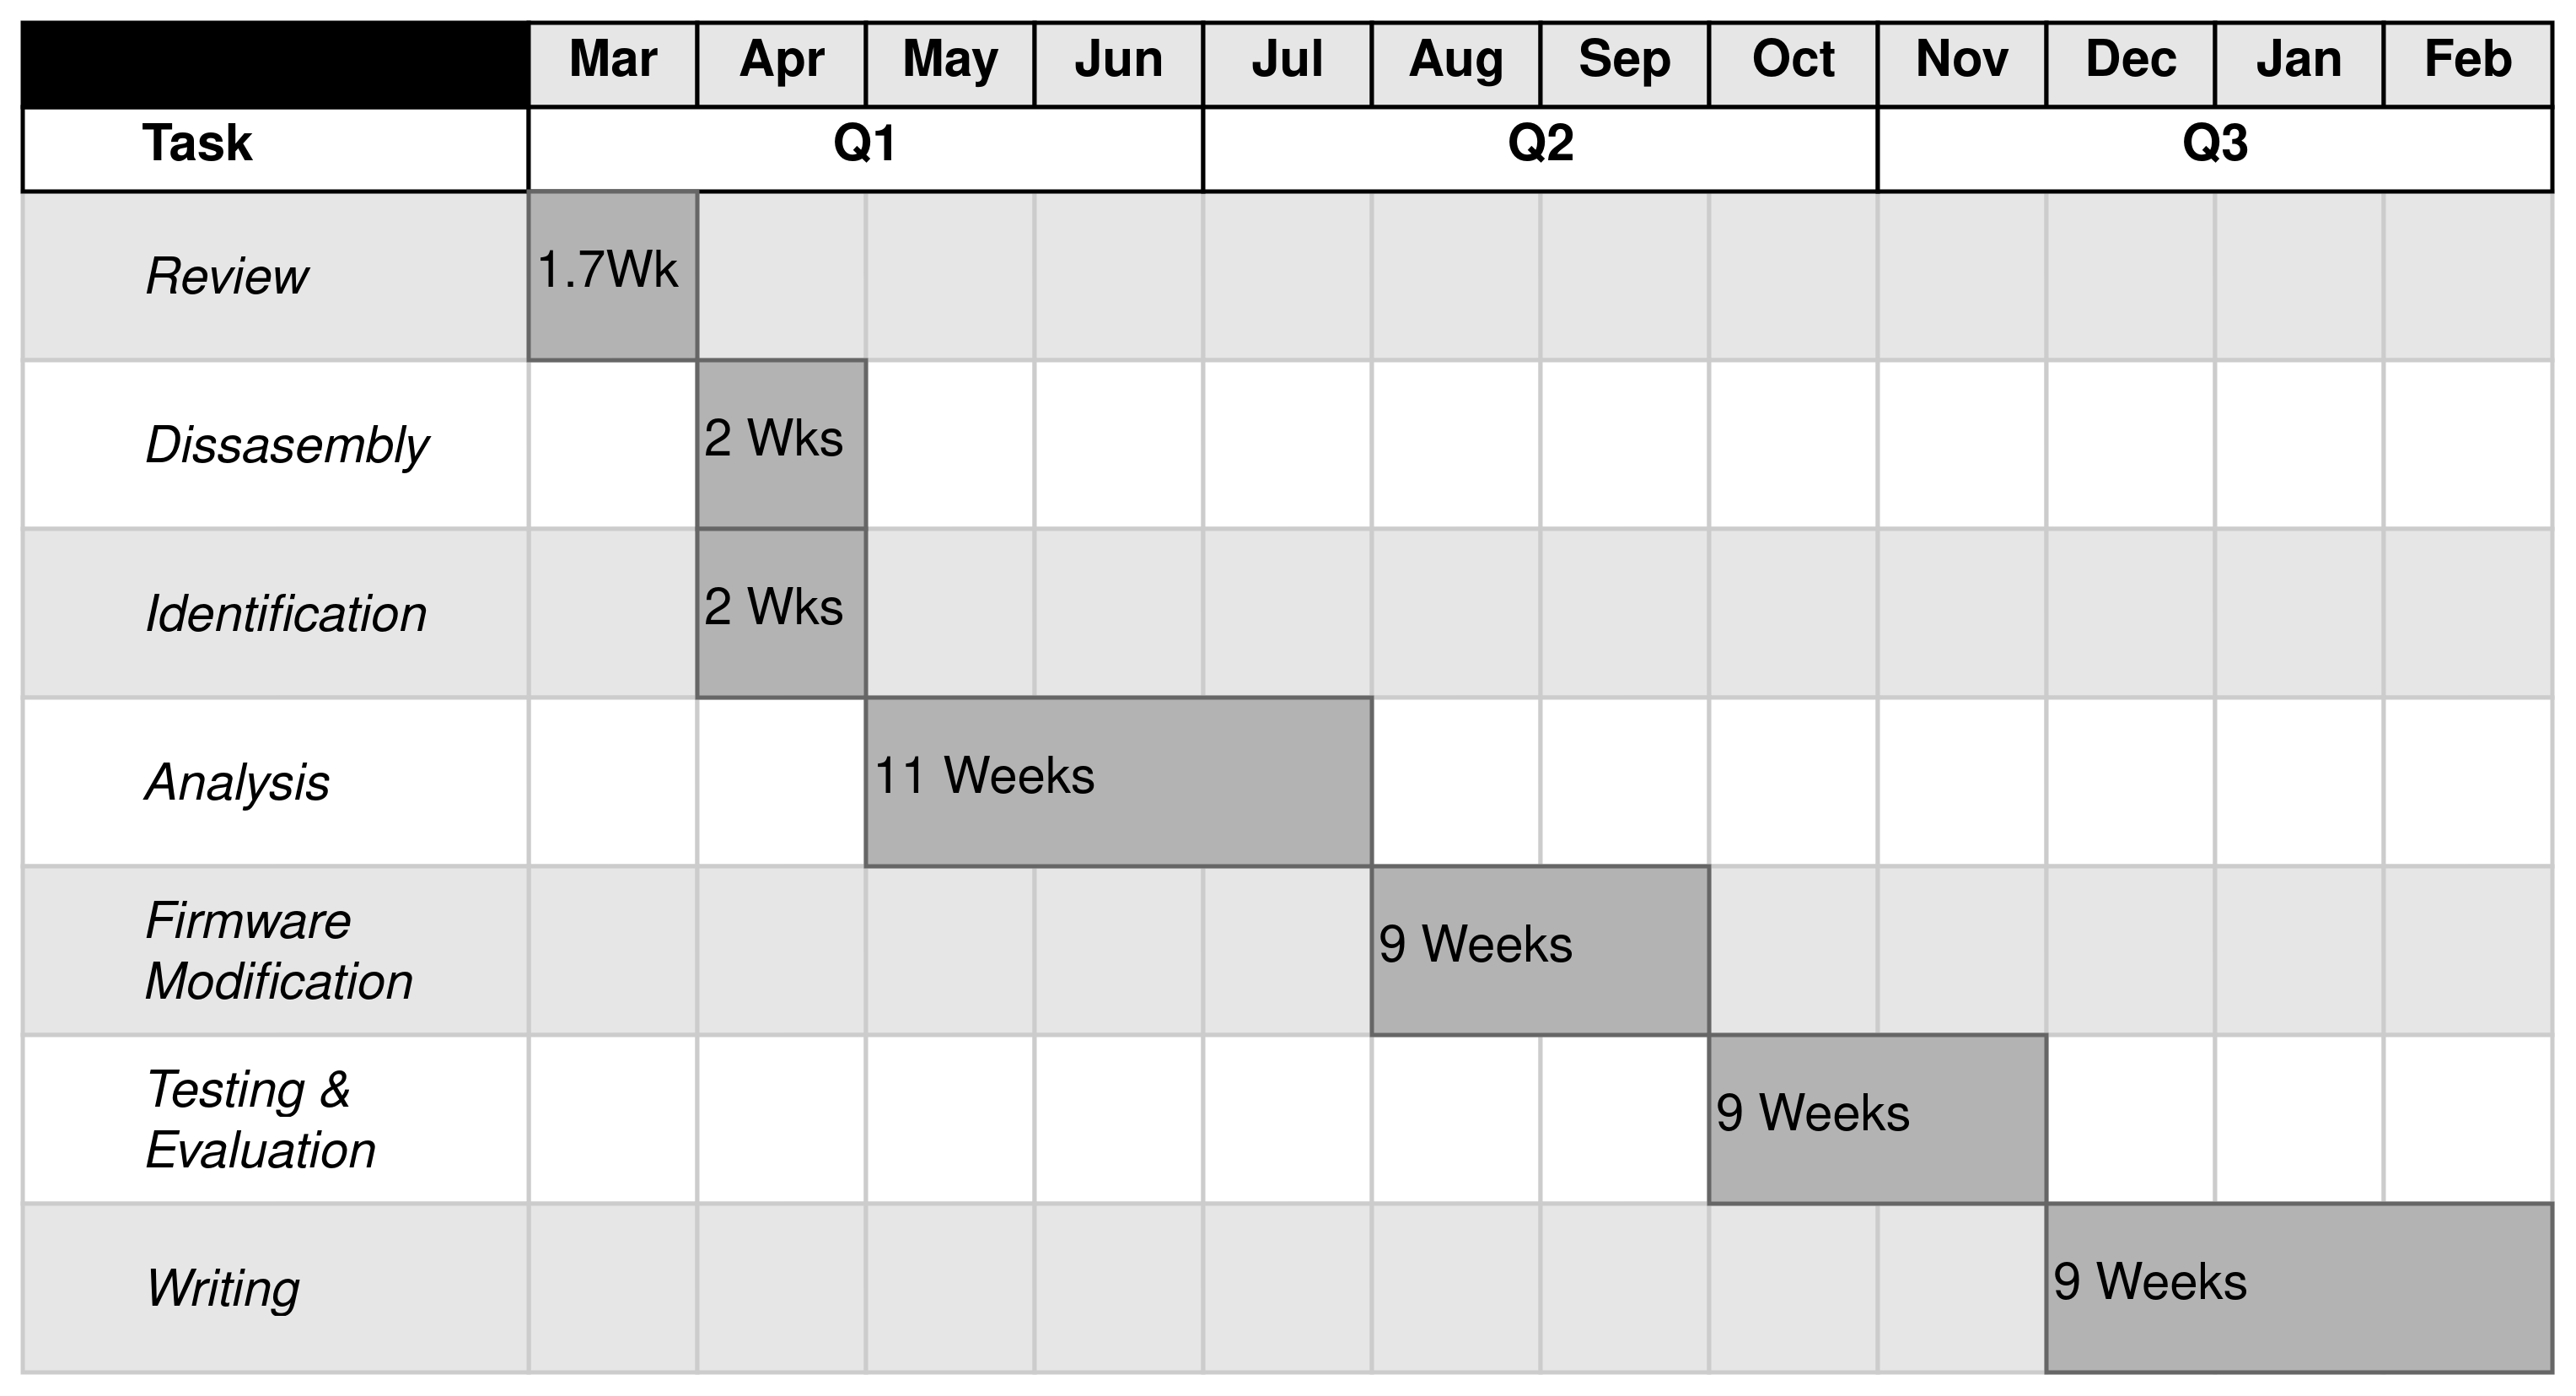
\includegraphics[width=160mm,scale=1]{Figures/timeline_gantt.drawio.png}}
  \caption{Research lifecycle}%
  \label{fig:research_lifecycle}%
\end{figure}

The timeline for the research proposal is divided into seven parts: review, disassembly, identification, analysis, firmware modification, testing, and writing. The dates provided are rough estimates and will vary as the project progresses. If any part of the process needs more time, there is a bank of four weeks that can be used and is already accounted.

% \begin{itemize}
%   \item \textbf{Review}: Review the proposal before beginning the research process to familiarize with the defined methodology, processes, and scope of project.
%   \item \textbf{Surveying}: Gather the necessary technical data and acquire the devices.
%   \item \textbf{Disassembly}: Each device is torn down, components identified, and documented.
%   \item \textbf{Writing}: All data collected, pictures taken, and documents created will be gathered to create a formal report as dictated by the research purpose.
% \end{itemize}

% \begin{table}[h]
%   \centering
%   \begin{tabular}{ |l||c|c|c| }
%     \hline\rowcolor{gray!30}

%     \textbf{Task} & \textbf{Duration} & \textbf{Start Date} & \textbf{End Date} \\
  
%     \hline

%     % creates empty row
%     % &  &  &  \\
%     % \multicolumn{4}{|c|}{} \\

%     \hline\rowcolor{gray!10} 

%     \textbf{Review} & 7 days & 24 Mar 25 & 30 Mar 25 \\

%     Review proposal comments/feedback & 2 days & 24 Mar 25 & 25 Mar 25 \\
%     Amend any changes & 3 days & 26 Mar 25 & 28 Mar 25 \\
%     Prepare work environment & 2 days & 29 Mar 25 & 30 Mar 25 \\

%     \hline
%     \hline\rowcolor{gray!10} 

%     \textbf{Disassembly} & 7 days & 31 Mar 25 & 06 Apr 25 \\

%     Disassemble printer & 2 days & 31 Mar 25 & 01 Apr 25 \\
%     Document interior/exterior of device & 5 days & 02 Apr 25 & 06 Apr 25 \\

%     \hline
%     \hline\rowcolor{gray!10}

%     \textbf{Identification} & 7 days & 07 Apr 25 & 13 Apr 25 \\

%     Identify device components & 3 days & 07 Apr 25 & 09 Apr 25 \\
%     Attempt hardware debug & 1 days & 10 Apr 25 & 10 Apr 25 \\
%     Identify software/hardware protections & 2 days & 11 Apr 25 & 12 Apr 25 \\
%     Document & 1 days & 13 Apr 25 & 13 Apr 25 \\

%     \hline
%     \hline\rowcolor{gray!10}

%     \textbf{Analysis} &  76 days & 14 Apr 25 & 29 Jun 25 \\

%     Capture network/USB traffic & 7 days & 14 Apr 25 & 20 Apr 25 \\
%     Analyze network/USB traffic & 31 days & 21 Apr 25 & 21 May 25 \\
%     Analyze recovered firmware & 31 days & 22 May 25 & 22 Jun 25 \\
%     Document previous tasks & 7 days & 23 Jun 25 & 29 Jun 25 \\

%     \hline
%     \hline\rowcolor{gray!10}

%     \textbf{Firmware Modification} & 62 days & 30 Jun 25 & 31 Aug 25 \\

%     Modify existing firmware & 31 days & 30 Jun 25 & 31 Jul 25 \\
%     Modify third-party firmware & 31 days & 01 Aug 25 & 31 Aug 25 \\

%     \hline
%     \hline\rowcolor{gray!10}

%     \textbf{Testing} & 60 days & 01 Sep 25 & 31 Oct 25 \\

%     Setup testing environment & 7 days & 01 Sep 25 & 07 Sep 25 \\
%     Reflash device w/ modified firmware & 14 days & 08 Sep 25 & 21 Sep 25 \\
%     Test print operations & 7 days & 22 Sep 25 & 28 Sep 25 \\
%     Test HID attacks & 7 days & 29 Sep 25 & 05 Oct 25 \\
%     Make changes and retest & 25 days & 06 Oct 25 & 31 Oct 25 \\

%     \hline
%     \hline\rowcolor{gray!10}

%     \textbf{Extra} & 30 days & 01 Nov 25 & 30 Nov 25 \\
    
%     \hline
%     \hline\rowcolor{gray!10}

%     \textbf{Writing} & 62 days & 01 Dec 25 & 31 Jan 25 \\

%     % \hline
%     % \hline\rowcolor{gray!30}
%     % \textbf{Entire research process} & 42 days & 06 Nov 25 & 18 Dec 25 \\

%     \hline
%   \end{tabular}
%   \caption{Research lifecycle}
%   \label{fig:research_lifecycle}%
% \end{table}
